\section{GameObjects(Ronan)}

\subsection{GameObjects in a game engine}
GameObjects are the fundamental entities that represent characters, props, lights, enemies and scenery.
GameObjects are essentially containers for components, which implement the GameObject's functionality.
\\\\
\noindent A few examples of components a GameObject might have are:
\begin{itemize}
    \item \textbf{Transform component:}
          A component handling the position, rotation and scale of a GameObject.
    \item \textbf{Render component:}
          A component to display a GameObject.
    \item \textbf{Physics component:}
          A component to add physics to a GameObject, for example velocity and mass.
    \item \textbf{Script component:}
          A component to define the behaviour of a GameObject.
    \item \textbf{Collider component:}
          A component to detect and respond to collisions with the GameObject.
\end{itemize}

\noindent GameObjects are always part of a scene and can interact with each other through the added components.

\subsection{Adding components to game objects}
A GameObject is just an empty vessel that needs components to be attached to it.
To add components to a GameObject, the following steps have to be taken:
\begin{enumerate}
      \item \textbf{Defining components:}
            Components are derived from a base or interface class to ensure each component is managed in a uniform way.
            Each component will hve a specialized role, like rendering or physics.
      \item \textbf{Attaching components:}
            When a component is added to a GameObject, the engine ensures that the component integrates correctly with 
            the GameObject and other components that are already attached. Some components need another component to function.
            An example of this is the Collider component, which needs a Transform component.
      \item \textbf{Limiting component types:}
            GameObjects can have multiple components, but most components should be limited to one per game object.
            An example of this is the Physics component, which should be limited to one component to prevent conflicting behaviour.
\end{enumerate}

\noindent Adding components to GameObjects this way also includes the ability to add or remove components dynamically.
This opens up the possibility for changes in a GameObject's behaviour during gameplay.
\\
Removing components is also important for GameObjects.
The engine should be able to detach and dispose of components when they are no longer needed.
This will lead to less resource usage.

\subsection{General architecture for GameObjects and Components}
There are several ways to build up the architecture for components and GameObjects:

\subsubsection{Entitity Component System}
Entity Component System, or ECS, is an architectural pattern that separates data from behaviour.
ECS works with the composition over inheritance principle, which provides improved flexibility and helps developers more easiliy
identify entities in a game scene.

\noindent ECS consist of the following elements:
\begin{itemize}
      \item \textbf{Unique identifiers known as entities}
            Entities are a distinct object that represent a GameObject.
            Entities are commonly expressed as a unique integer value.
            Entities contain no data or behaviours.
            Entities may contain zero or more components.
            Entities can dynamically change components.
      \item \textbf{Plain datatypes without behaviour known as components:}
            Components are datatypes consisting or unique behaviour assigned to an entity.
            They are reusable modules that can be attached to entities.
      \item \textbf{Systems which are matched with and entities that contain a particular set of components:}
            Systems iterate components to perform functions like updating the components with for example physics calculations.
            System provide the global scope, services and managing for components classes.
\end{itemize}

\noindent An example of how example of how ECS might be used in a game engine can be seen in the following picture:
\begin{figure}[h!]
      \centering
      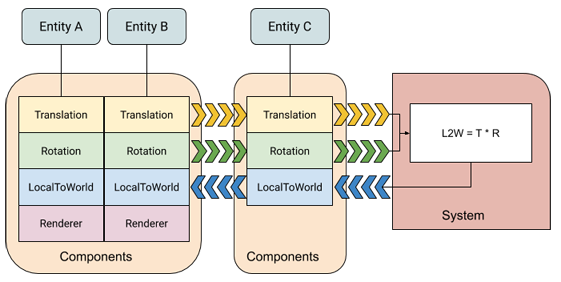
\includegraphics[width=0.6\textwidth]{ECSBlockDiagram.png}
      \caption{ECS Block diagram}
      \label{fig:ECSBLockDiagram}
\end{figure}
\newpage

\noindent \textbf{Advantages:}
\begin{itemize}
      \item ECS can be used to create shorter and less complicated code.
      \item ECS offers a clean design using decoupling, encapsulation en modularization.
      \item ECS lets developers use reusable parts.
      \item New features can be added more easiliy.
      \item Data and logic are seperated.
      \item ECS is multi-threading friendly.
      \item ECS is great for efficiently managing large-scale systems with many enitities.
\end{itemize}

\noindent \textbf{Disadvantages:}
\begin{itemize}
      \item ECS is not as concretely defined as other patterns.
      \item ECS is challenging to apply correctly and can be misused easily. It is more complicated to design and implenent correctly than other methods.
      \item ECS requires a lot of small classes which can potentially be used in a large number of entities. There is a risk of writing inefficient code.
\end{itemize}
\cite{simplilearn}

\subsubsection{Object-Oriented with Extensions}
With an Object-Oriented design using Extensions, a middleground is achieved between traditional Object-Oriented inheritance and more modular/compositional designs.
It allows developers to take advantage of inheritance, encapsulation and polymorphism while maintaining flexibility through the use of Extensions.

\noindent There are a few key concepts of an Object-Oriented design using Extensions:
\begin{itemize}
      \item \textbf{Core GameObject class:}
            A core GameObject which holds essentially data like an ID and a name.
      \item \textbf{Extensions using composition:}
            Components are attached to GameObjects dynamically using Extensions, without the GameObject knowing the details of the components.
            Component are reusable for different GameObjects.
      \item \textbf{Changing components dynamically:}
            Components can be added, modified or removed during runtime, which is more flexible than a standard Object-Oriented architecture. 
\end{itemize}

\noindent A big difference between this architecture and ECS, is that components do contain logic and not just data.
\\\\
\noindent \textbf{Advantages:}
\begin{itemize}
      \item Easy to implement as it uses the familiar OOP structure.
      \item Seperation of concerns, logic is separated from GameObjects.
      \item Components can be added, removed and modified dynamically.
      \item Components can be reused for different GameObjects, which avoids deep inheritance.
      \item In simpler games, it can provide a more straightforward architecture compared to ECS.
\end{itemize}

\noindent \textbf{Disadvantages:}
\begin{itemize}
      \item Danger of tight coupling between Extensions and GameObjects.
      \item This architecture can struggle in large games where lots of GameObjects need to be processed.
\end{itemize}

\textbf{TO DO:}
Meer patterns onderzoeken?
Extensions uitbreiden?
References fixen